\documentclass[conference]{IEEEtran}
\usepackage{amsmath,amsfonts,amssymb}
\usepackage{graphicx}
\usepackage{color}
%\usepackage{url}

\begin{document}
\title{CS8803-O03 Reinforcement learning\\Project 2 report}

\author{\IEEEauthorblockN{Rohan D. Kekatpure}
\IEEEauthorblockA{Email: rdk@gatech.edu}}
% make the title area
\maketitle

% As a general rule, do not put math, special symbols or citations
% in the abstract
%\begin{abstract}
%\end{abstract}

\IEEEpeerreviewmaketitle
\section{Introduction}
The aim of this project is to train a reinforcement learning (RL) agent in a discrete-action continuous-state-space environment. The chosen agent is the lunar lander in the Box-2D environment. This project brings together many aspects of RL and the course together. The project is a miniature version of latest advances in the field of RL. As such, despite the pain and nearly 100+ hours spent on this project, it has forced synthesis of the class material.
%%
\section{implementation methodology}
\subsection{Overview}
Our implementation for this project is a simplified version of the methodology presented in the DQN paper\cite{dqn}. While the RL part of the overall algorithm is identical to Algorithm 1 in the paper, our function approximation technique differs in from the DQN implementation in two important ways: (1) we use a simple, fully connected feed-forward neural network for function approximation (as opposed to convolutional net (CNN) in the DQN paper) and (2) we our total ``state'' is a combination of the 8-component state provided by the environment and the {\bf one-hot-encoded} action vector. 
%%
\subsection{Choice of hyperparameters}
\begin{enumerate}
\item
{\bf Exploration probability $\epsilon$:} We employed a TD(0)-like RL algorithm with an $\epsilon$-greedy exploration strategy. The parameter $\epsilon$ is initialized at 1.0 and is decayed by 1\% ($\epsilon_{\text{decay}} = 0.99$) at each step until it reaches a minimum of 0.1. The motivation to keep exploring is to avoid being stuck in local maxima. One local optimum we observed in the training of our agent was when the agent avoids landing. To avoid crashing with a reward of -100, it keeps firing the main engine until the end of episode. The particular value of $\epsilon_{\text{decay}} = 0.99$ keeps the probability of exploration $>10\%$ until 100 episodes. The DQN paper uses similar (though not identical) values.

\item
{\bf Discount factor $\gamma$:} We found that lunar lander episodes last on average for a 100--500 steps. So the RL horizon is practically finite and we do not expect $\gamma$ to impact the solution very much. We therefore started our experiments with $\gamma=0.99$ and found that this value led to convergence. We repeated the experiments for values $0.70\leq \gamma \leq 0.99$ and found little effect on the convergence behavior.

\item
{\bf Replay memory and training batch size:} After our failed experiments with batch-mode updates using states in a single episode, we settled on batching and experience replay as recommended in the DQN paper. We noticed that training with states from a single episode makes the weights diverge. For our agent we fixed replay memory at 50000 and the batch size at 32. Once again we found no appreciable difference in convergence or stability for batch sizes of $\{32, 64, 128\}$, but the speed of computation increases with decreasing batch sizes.
 
\item 
{\bf Learning rate $\alpha$:} The learning rate crucially affects the convergence of $Q$ learning. We chose a {\bf constant} learning rate of $\alpha = 10^{-4}$ by logarithmically varying it from $10^{-5}$ to $10^{-2}$. Our chosen value offered a fast monotonic convergence.

\item 
{\bf Neural net training epochs per episode:} We train our neural net at each step of every episode. Allowing the neural net training to run for the default number of  epochs (200 in sklearn's {\tt MLPRegressor}) not only increases the training period, but also {\bf overfits} to a particular batch. To speed up training significantly and to avoid overfitting, we fixed number of training epochs per episode to 2. 
\end{enumerate}
%%
\subsection{Neural net structure}
We use a simple feed-forward neural network (motivation in \S~\ref{sec:expts1}) with two hidden layers of 50 nodes each and rectified activation. Our output layer is a single neuron without any activation. As mentioned previously, the network is trained with a constant learning rate of $\alpha=10^{-4}$. As a result of fusing the raw state with (encoded) action vector, our implementation needs to do 4 passes for the ``prediction'' part. The chosen ``action'' is the one that maximizes the output value.
%%
\subsection{Software dependencies}
Our solution is implemented within standard Python ecosystem; the only external dependencies are numpy and scikit-learn. In particular, we {\bf don't} use high-performance neural network learning frameworks such as Theano or Tensorflow, or their wrappers like Keras. 
%%
\section{Experiments}
\subsection{Choice of learner}\label{sec:expts1}
RL success stories (TD-Gammon, Atari, Go) leave little doubt about the efficacy of neural nets as the function approximators. Yet, it is not obvious (at least to this author) why other supervised algorithms would not be able to outperform neural nets. To test the strength of other supervised algorithms on RL tasks, we experimented with linear, SVM and decision tree learners (regressors). Table~\ref{tab:learners} summarizes the maximum average reward per 100 episodes that these learners were able to achieve. 

Our empirical evidence, though not exhaustive, hints to superiority of neural nets over other learning algorithms for $Q$ function generalization. One reason might be the non-linearity coupled with extreme non-convexity in the $Q$ function landscape. As a result, linear regression may have insufficient flexibility (i.e. high bias) to approximate the $Q$ function. Regression trees are provably {\bf universal function approximators}. In theory they have equal expressive power as neural nets. Yet, in practice it may be difficult to search the hypothesis space efficiently in decision-tree representation. In addition, the hidden layers in neural nets have been interpreted to be representations of latent information in raw features (e.g. ``face-like'' or ``nose-like'' etc). This made it clear that we needed the expressive power of a neural net for $Q$-function approximation for this task.
%%
\begin{table}[bpht]
\begin{center}
\begin{tabular}{|l|c|l|}
\hline
Learner & Max avg. reward & sklearn params \\ \hline 
Linear regression & $<-200$ & -\\
SVM & $<-170$ & $C=0.01, \epsilon=0.2$ \\
Regression tree &$<-115$ & tree depth $\leq 15$ \\
Neural net & $> +55 $ & layers = $(50, 50), \alpha =10^{-3} $ \\ \hline
\end{tabular}
\end{center}
\caption{Maximum 100-episode average reward achieved by different learners on $Q$ learning. \label{tab:learners}}
\end{table}
%%
\subsection{Neural net parameters}
One drawback of neural network is the requirement for fine tuning of a number of hyper parameters. We ran a small number of experiments to get a general idea of the number of {\bf layers}, number of {\bf nodes per layer}, number of {\bf epochs} and the {\bf batch size}. It is computationally a difficult task to perform extensive parameter sweeps, so the choice of experiments is somewhat arbitrary. 

The fixed parameters for our neural net were {\tt warm\_start=T}, {\tt fitting\_func=partial\_fit}, and ``adam'' as the SGD solver. As seen in Table~\ref{tab:nnarch}, the number of neural net training epochs per episode or larger number of hidden nodes don't necessarily lead to better fits. Reducing the epochs and hidden nodes does lead to significant speedup at the cost of a slight drop in max reward. As a result, out final neural net implementation used two hidden layers with {\bf 50 nodes} each, a {\bf 32 sample} batch size, and {\bf 2 epochs} per episode (1 epoch leads to underfitting). 
%%
\begin{table}[bpht]
\begin{center}
\begin{tabular}{|c|c|c|c|c|c|c|}
\hline
layers & epochs & solver & iters & batch & speed & max rew\\ \hline 
(50, 50) & 50 & ``adam'' & 1000 & 128 & slow & +124 \\
(100, 100) & 50 & ``adam'' & 1000 & 256 & slow & +85 \\
(50,50) & 20 & ``adam'' & 700 & 32 & ok & +132 \\
(50,50) & 2 & ``adam'' & 700 & 32 & fast & +90 \\ \hline
\end{tabular}
\end{center}
\caption{Maximum 100-episode average reward achieved by different neural net architectures. \label{tab:nnarch}}
\end{table}
%%
\subsubsection {Neural net training epochs}
We train our neural net at each step of every episode. Allowing the neural net training to run for the default number of  epochs (200 in sklearn's {\tt MLPRegressor}) not only increases the training period, but also {\bf overfits} to a particular batch. To speed up training significantly and to avoid overfitting, we fixed number of training epochs per episode to 2. Figure~\ref{fig:lr} demonstrates that a wrong choice of the training epochs can lead to training failure and unoptimized agents.
%%
\begin{figure}[tbp]
    \centering
    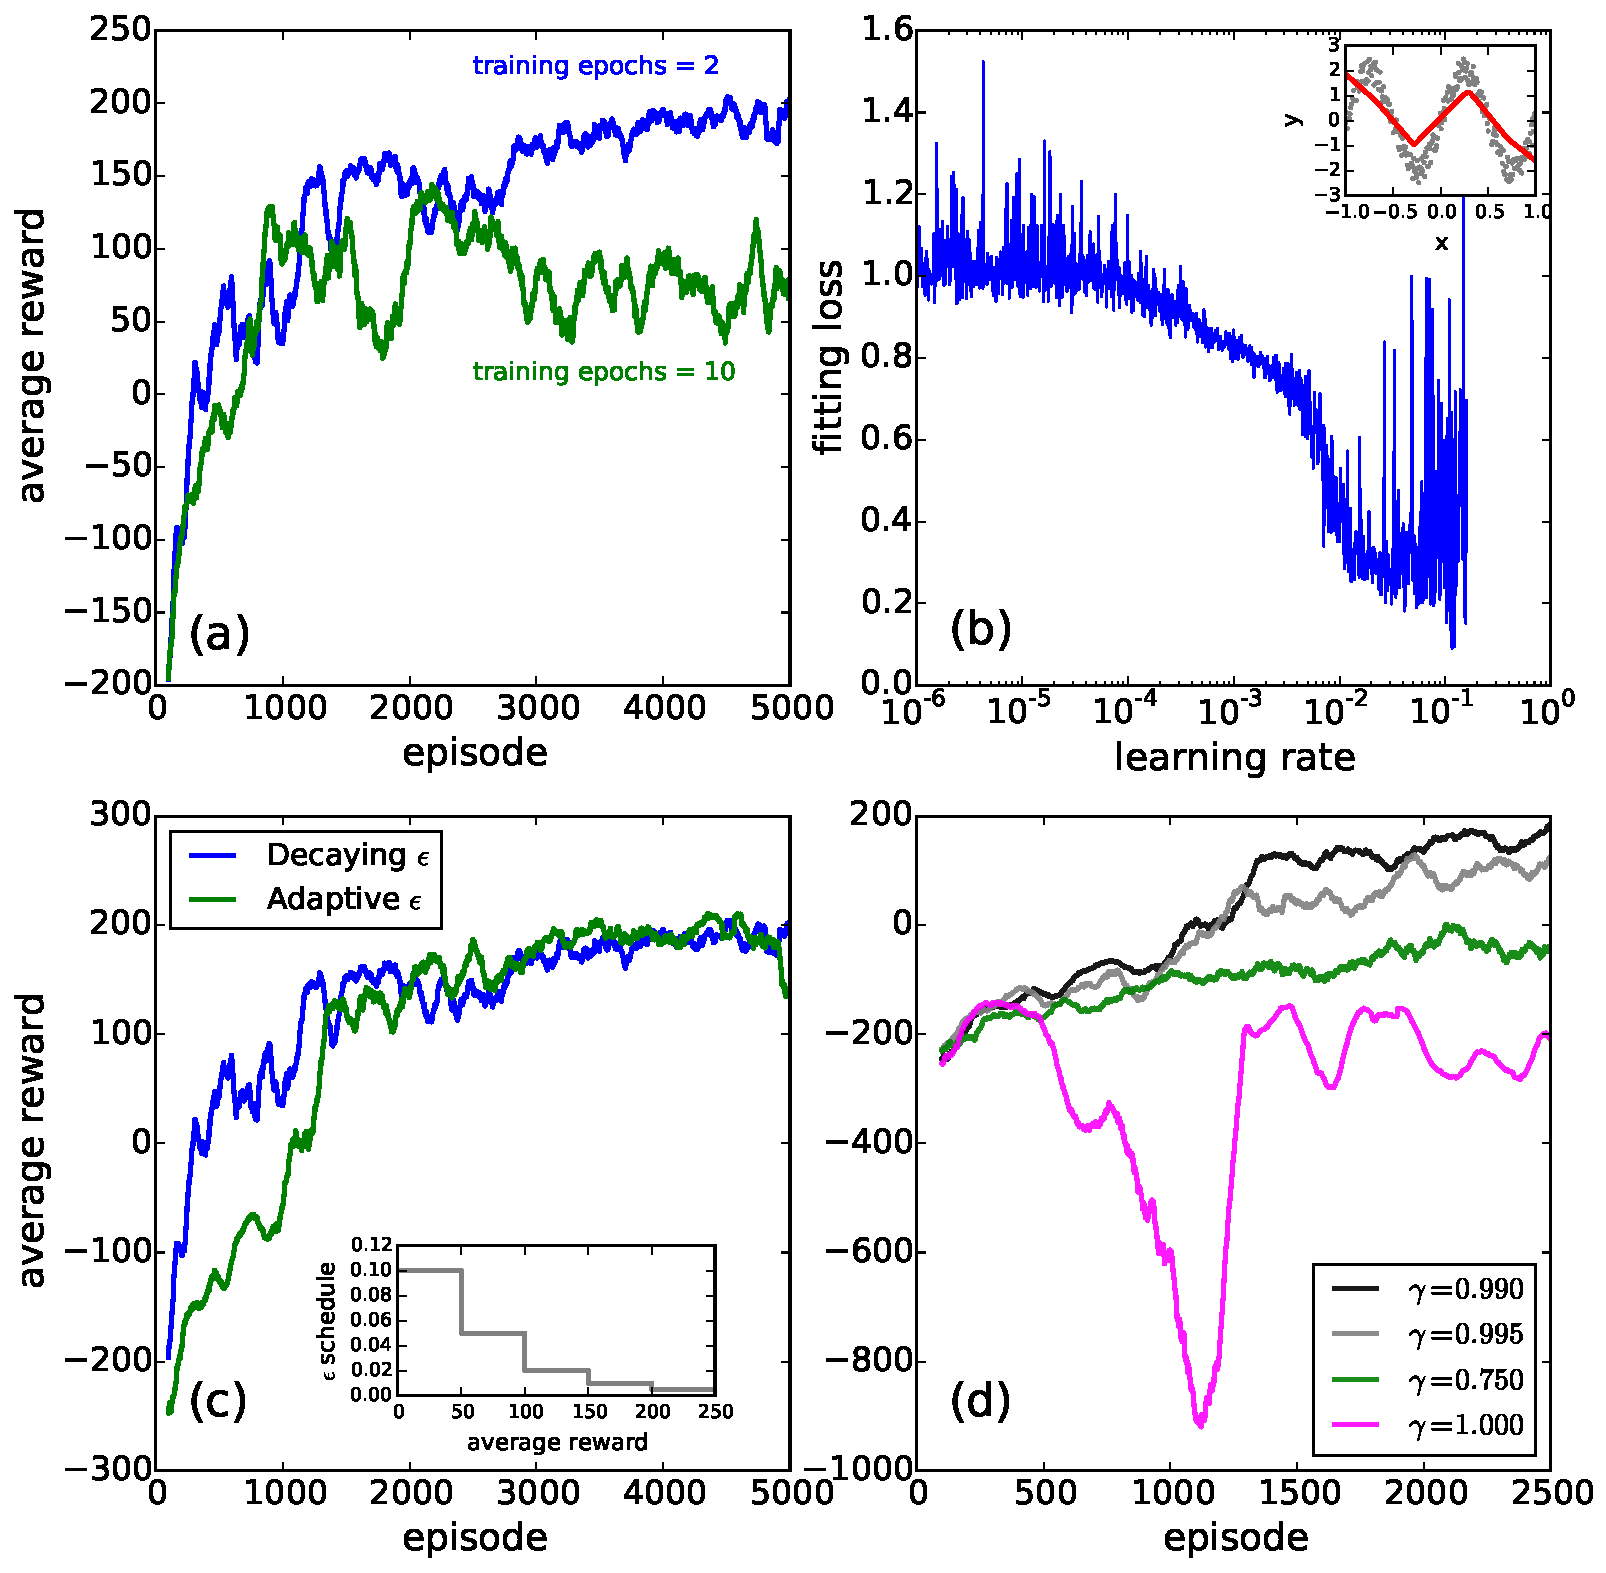
\includegraphics[width=0.5\textwidth]{./figures/fig0.pdf}
    \caption{(a) Agent training effectiveness vs epochs per episode. Optimal epochs per episode $\simeq 2$ (b) Learning rate vs fit quality for a simple 1D fit using our neural net regressor. Stable learning rate $\simeq \alpha=10^{-4}$ \label{fig:lr}}
\end{figure}
%%
\subsubsection{Learning rate}
We estimated the optimal range of the learning rate $\alpha$ by fitting a 3-period sinusoid (a proxy for a non-convex, nonlinear function) using the neural net fixed in the previous section. The learning rate vs the fit quality is plotted in Fig.~\ref{fig:lr}. It is clear that $\alpha>0.01$ can lead to unstable behavior even for this simple one-dimensional learning task. To keep the learning behavior stable we conservatively set our learning rate at a {\bf fixed } value of $\alpha = 10^{-4}$
%%
\section{Results}
\subsection{Behavior during training}
After the choice of hyper parameters, we ran the training of our agent for 20000 episodes. The reward for each episode during training for first 5000 episodes is plotted in Fig.~\ref{fig:fig1}. Although there are many early episodes with reward $>200$, they're chance occurrences. The agent is fully trained (average reward $>200$) only after episode 1165. We note that the training of the agent is fairly robust as signified by the relatively flat (though noisy) training curve.
\begin{figure}[tbp]
    \centering
    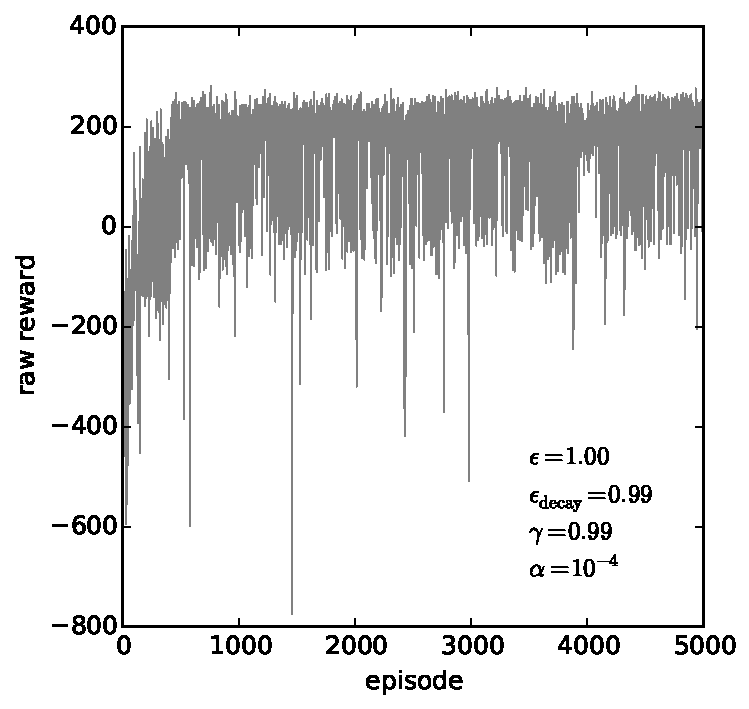
\includegraphics[width=0.5\textwidth]{./figures/fig1.pdf}
    \caption{Reward at each episode during agent training. \label{fig:fig1}}
\end{figure}
\subsection{Behavior after training}
Fig.~\ref{fig:fig2} shows the smoothened version of Fig.~\ref{fig:fig1}. We've also shown the entire 20000 training episodes to highlight regions of {\bf overfitting}. The average reward is stable and between 150 and 200  
%%
\begin{figure}[tbp]
    \centering
    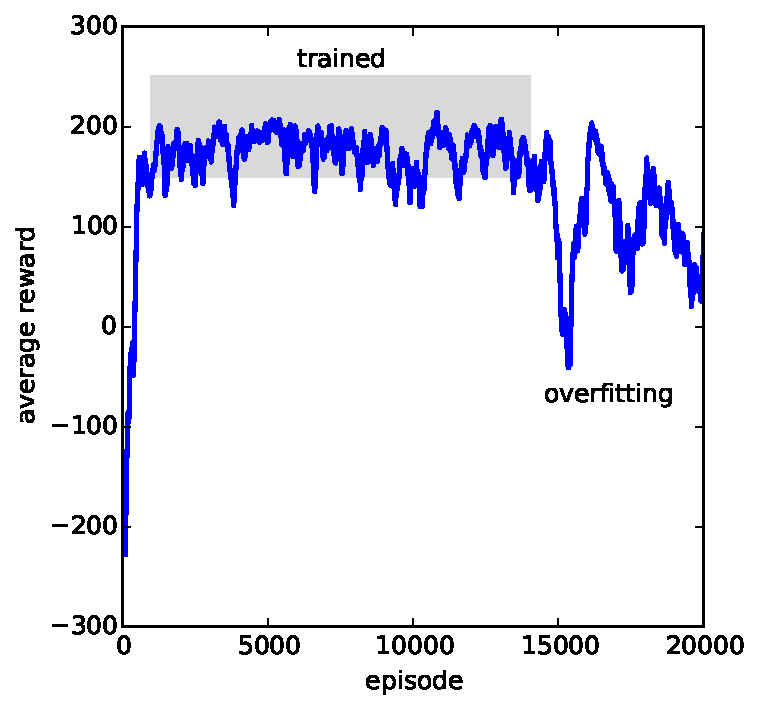
\includegraphics[width=0.5\textwidth]{./figures/fig2.pdf}
    \caption{100-episode average reward during training. The gray shaded region corresponds to a trained agent per the problem definition. \label{fig:fig2}}
\end{figure}
%%
\section*{Conclusion}
 
\begin{thebibliography}{1}
\bibitem{dqn}
V.~Mnih et al., ``Playing Atari with Deep Reinforcement Learning,'' {\em arXiv:1312.5602 [cs.LG]} 2013.
\bibitem{sutton88}
Richard~S.~Sutton, {\em Machine Learning}, {\bf 8} p. 9--44, 1988.
\bibitem{suttonbarto}
Richard~S.~Sutton and Andrew~G.~Barto, ``Reinforcement Learning,'' {\em MIT Press}, 1998.
\end{thebibliography}

\end{document}


